\chapter{BGP MRAI dependency}
\label{cha:bgp_mrai_experiments}

\ac{MRAI} is one of the parameters that mostly has caused divergences in the
scientific community.
And, after the introduction in the protocol in version 4~\cite{rfc4271},
is one of the parameter more studied for its multiple effects, the correct setting
can improve the protocol performances.
While, an incorrect one can generate exponential convergence behaviours even
in small network~\cite{fabrikant2011there,griffin2001experimental}.

The protocol strictly depends on this parameter, because, as showed in \Cref{cha:bgp_fsm},
the incorrect use of it can lead to tremendous consequences, even worst of not
having it at all.
In other cases, with a particular setting of it is possible to improve the network
performances.
Recent studies about centrality metrics on routing protocols introduce, through
the distributed computation of the metric, a
timer trade-off improvement~\cite{MaLo18_ToN,GhiMa18_infocom}.
This kind of approach has been also applied on \ac{BGP} with positive results on
network failures~\cite{milani2019BGP,milani2020improving}.

All those studies points out how we can set \ac{MRAI} to improve network
performances, but what about how \ac{MRAI} reacts to different problems?
Is it possible that \ac{MRAI} reacts differently based on where the signal
occurs?
In fact, our hypothesis is that is not enough just look to the \ac{MRAI} setting,
because, other factors can be relevant too.
For example, a change near the central clique of $T$ nodes could provoke a large
storm of messages because \ac{MRAI} doesn't affect in time the spreading of information.
While, a change in the periphery could be cushioned without it reaching the center
of the network multiple times.

\section{Different MRAI strategies}
\label{sec:bgp_mrai_strategies}

An \ac{MRAI} strategy define a particular way to set all the timers accordingly
to a set of rules or properties.
For example, the default strategy of \ac{MRAI}, defined in~\cite{rfc4271}, is
to set all the timers to \SI{30}{\second}.
In \cref{sec:bgp_fsm_experiments} I used \num{4} different \ac{MRAI} strategies
to show that an incorrect setting of it can lead to dangerous consequences.
Another strategy that can be used during some experiments is the complete avoidance
of it, this is the \emph{NoMRAI} technique.

The hypothesis behind all the different strategies is that is possible to
adjust the trade-off between the network performances adapting this timer.
Recent studies try to use the centrality to adapt \ac{MRAI} using the position
of the node as property~\cite{milani2020improving}.

\subsection{Centrality based strategy}
\label{subsec:bgp_mrai_dpc}

The centrality based strategy is inspired from the \textit{PopRouting} idea
that has been successfully implemented in other protocols~\cite{MaLo18_ToN,GhiMa18_infocom}.
The idea behind those studies is to exploit the fact that the more central nodes
in the network should be more reactive to changes while the nodes that resides
in the border of the network don't have a major influence.
Load centrality and betweenness centrality are examples of centrality metrics
that can be calculated on a graph~\cite{Brandes2008variants}, the load centrality
is defined as follow.

\begin{definition}[Load Centrality]
		Consider a graph \graph and an algorithm to identify the (potentially multiple)
		minimum weight path(s) between any pair of vertices $s,d$.
		Let $\theta_{s,d}$ be a quantity of a generic commodity that is sent from vertex
		$s$ to vertex $d$.
		We assume the commodity is always passed to the next hop following the minimum weight paths.
		In case of multiple next hops, the commodity is divided equally among them.
		We call $\theta_{s,d}(v)$ the amount of  commodity forwarded by vertex $v$.
		The \emph{load centrality} of $v$ is then given by:
		\begin{equation}
				LC(v) = \sum_{s,d \in \nodeset}\theta_{s,d}(v)
				\label{eq:lc}
		\end{equation}
\end{definition}

This mechanism is compatible with network protocols where there is an exchange
of messages that accept the introduction of the commodity.
In \ac{BGP} is possible to include optional attributes inside the \ac{ADV} messages.
For this reason I have created the \ac{DPC} and demonstrated that is possible
to calculate it in a distributed way~\cite{milani2019BGP} with small changes
to the protocol.

The \ac{DPC} better adapt to \ac{BGP} because it doesn't relay on the assumption
that every node must distribute a load.
The number of network prefixes distributed represent the load introduced on a
network by a node.
Not all \ac{BGP} speakers distribute an \ac{IP} prefix, but every node that forward
traffic have a non-zero \ac{DPC} centrality value.

We call $\destinationset \subseteq \nodeset$ the set of nodes that can be source
and/or destination of traffic (they export at least one network)
and $N_s, N_d$ the number of networks that are exported by node $s$ and $d$,
respectively, then $\theta_{s,d} = \frac{N_s + N_d}{2}$. \ac{DPC} $\Delta(v)$ of
any vertex $v\in \nodeset$ is defined as:
\begin{equation}
		\dpc(v) = \sum_{s,d\in \pathset} \theta_{s,d} (v)
		\label{eq:dpcv}
\end{equation}

Is then possible to configure \ac{MRAI} accordingly with the centrality metric
described, as has been done in~\cite{milani2020improving}.
I assume that the information in the \ac{ADV} messages propagates in the network
in three phases, identifying three propagation graphs:
\begin{itemize}
    \item \textit{\textbf{Ascending phase graph \ascentgraph}:} made by the
        nodes updated without reaching tier one nodes;
    \item \textit{\textbf{Tier one graph \tiergraph}:} made by tier-1 nodes;
    \item \textit{\textbf{Descending graph phase $\descentgraph = \graph - \ascentgraph - \tiergraph$}:}
        the rest of the graph.
\end{itemize}

Considering a graph-wide maximum timer $T=\SI{30}{\second}$ and \ac{DPC}
$\dpc(i) \in [0,1]$ for node $i$, DPC-based \ac{MRAI} $T_{ij}$ used by node $i$
with neighbor $j$ is set as follows:
\begin{equation} \label{eq:dpc}
    T_{ij}=
    \begin{cases}
        \frac{T}{2}\dpc(i) & \forall i\in \ascentnodeset  \\
    \frac{T}{2} & \forall i\in \tiernodeset \\
        \frac{T(1-\dpc(i))}{2}+\frac{T}{2} & \forall i\in \descentnodeset\\
    \end{cases}
\end{equation}

\subsection{Strategy comparison}
\label{subsec:bgp_mrai_strategy_comparison}

In order to make every strategy comparable is possible to adapt the timers to
respect a given $MRAI_{mean}$ value.
Given $M$ as the set of all the timers used in the network defined as follow:

\[M=\{T_{ij} | \forall (i,j) \in \edgeset\}\]

The average value of \ac{MRAI} is represented by \(M_{avg}=\frac{\sum_{m\in M} m}{\edgeset}\).
Given \(M_{avg}\) and the required \(MRAI_{mean}\) is possible to define
\(k=\frac{MRAI_{mean}}{M_{avg}}\).
Giving us the possibility to adapt \(M\) in order to respect \(MRAI_{mean}\)
multiplying each element of \(M\) by \(k\).

\[M^k=\{T_{ij}k | \forall (i,j) \in \edgeset\}\]

\section{Clique Experiments}
\label{sec:bgp_mrai_clique}

The clique topology is one of the worst-case scenarios as specified in Labovitz et al.~\cite{labovitz2000delayed}.
For this reason I decided to start my study from it.
I used two approaches in this Environment, the first one keeps the \ac{IW} active
the second one doesn't use this mechanism.
This to emphasize the effects of this mechanism with the influence also of different
\ac{MRAI} configurations.

The Environment properties are listed in \Cref{tbl:clique_properties}

\begin{table}[h]
	\begin{center}
	\begin{tabular}{ || m{4cm}| m{8cm} || } 
	\hline
	Property & Value \\ 
	\hline \hline
	Seeds & $[1, 10]$ \\ 
	\hline
	Signaling & \q{AW} \\
	\hline
		Withdraws delay & Uniform distribution between \SI{1}{\second} and \SI{5}{\second} \\ 
	\hline
	Announcement delay & constant distribution of \SI{5}{\second} \\ 
	\hline
		MRAI & $[0, 60]$ \\
	\hline
	Link delay & Uniform distribution between \SI{0.0001}{\second} and \SI{0.5}{\second} \\
	\hline
	\end{tabular}
\end{center}

		\caption{Clique environment properties, \num{10} possible different runs}
    \label{tbl:clique_properties}
\end{table}

As described in \Cref{tbl:clique_properties}, for each \ac{MRAI} value has been
executed \num{10} different runs of the environment.
The clique graph used in these experiments is composed by \num{15} nodes.
The \ac{MRAI} strategy used is the \textit{fixed} one, so every link will have the
same \ac{MRAI} value.
The results are presented in \Cref{fig:clique_evolution}

\begin{figure}[h]
     \centering
     \begin{subfigure}[b]{0.49\textwidth}
         \centering
         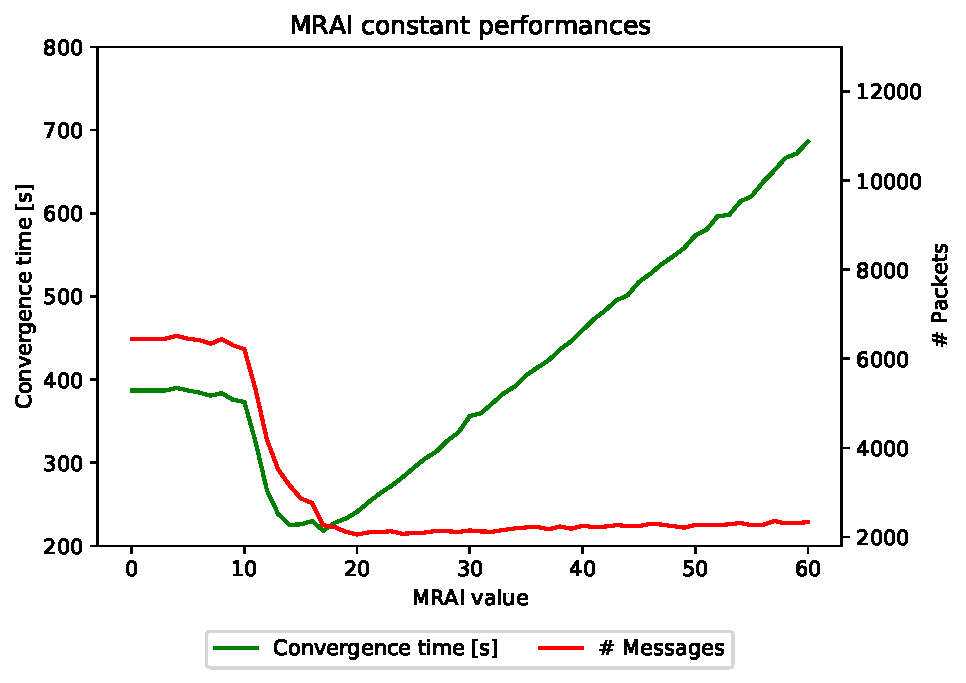
\includegraphics[width=\textwidth]{images/clique/messagesVStime/pareto-clique-constant_mrai_evolution.pdf}
		 \caption{Network performances \textbf{with} \textbf{\ac{IW}}}
         \label{fig:clique_evolution_IW}
     \end{subfigure}
     \hfill
     \begin{subfigure}[b]{0.49\textwidth}
         \centering
         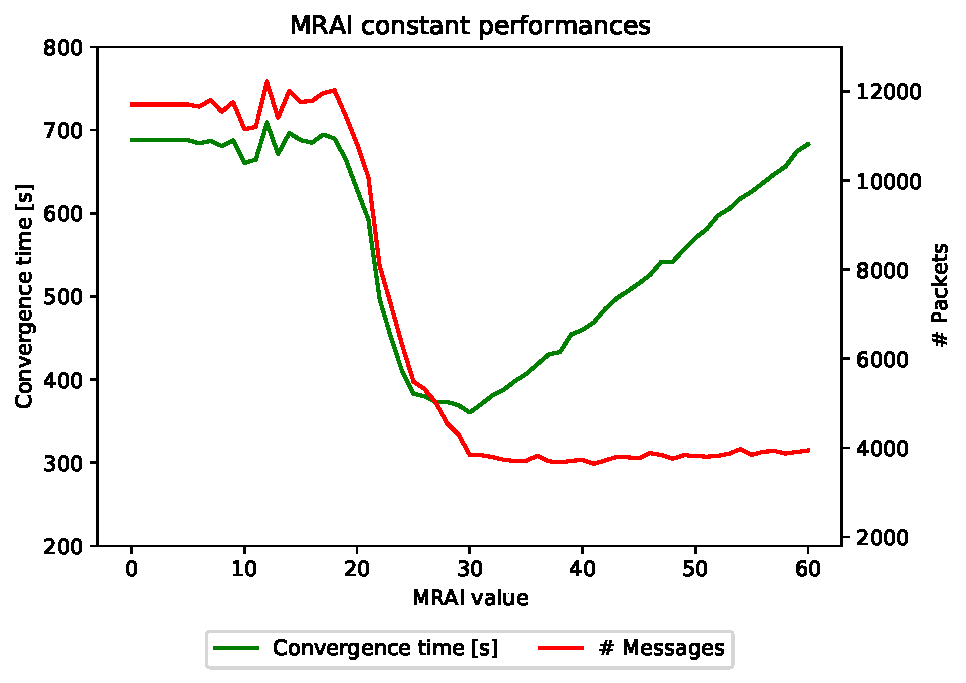
\includegraphics[width=\textwidth]{images/clique/messagesVStime/pareto-clique-noIW-constant_mrai_evolution.pdf}
		 \caption{Network performances \textbf{without} \textbf{\ac{IW}}}
         \label{fig:clique_evolution_noIW}
     \end{subfigure}
		\caption{Evolution of the network performances on the clique graph of \num{15}
			nodes using a fixed \ac{MRAI} from \num{0} to \num{60} seconds.
			Each point is the average of the \num{10} different runs provided
			by the environment in \cref{tbl:clique_properties}}
        \label{fig:clique_evolution}
\end{figure}

In \Cref{fig:clique_evolution} is possible to notice both the effect of \ac{MRAI}
and \ac{IW}.
Those plots represent the network performances in terms of convergence time and
number of messages transmitted to reach the convergence after the transmission
of the signal \q{AW}.
Each point in the plots is the average of the \num{10} runs executed with the
\textit{Fixed} \ac{MRAI} value on the $x$ axis.
The left $y$ axis should be used with the convergence time, the green line, while
the second $y$ axis represents the number of messages transmitted, the red line.
The convergence time represent the average convergence time of the entire network,
a node is considered converged when its \ac{RIB} doesn't change anymore.

The effects of \ac{MRAI} are present in both the plots but in two different
moments.
In \Cref{fig:clique_evolution_IW} \ac{MRAI} affects both the convergence time and
the number of messages around \SI{10}{\second} up to \SI{20}{\second}.
After the threshold of \SI{20}{\second}, the effects of \ac{MRAI} are counterproductive,
the convergence time is negatively affected because the nodes start to wait more
time without obtaining more useful information.
This can be seen also in the number of messages that reaches a constant value.
Other messages are not necessary to converge and \ac{MRAI} doesn't compress
the input anymore, so the nodes are not able to aggregate more information.

In \Cref{fig:clique_evolution_noIW} is possible to see the same effects but after a higher
\ac{MRAI} threshold.
The number of transmitted messages reaches the constant value with an \ac{MRAI}
value around \SI{30}{\second}.
The effects of \ac{IW} can be saw also in the number of messages and the convergence
time with a low \ac{MRAI}.
In \Cref{fig:clique_evolution_noIW} is possible to reach even \num{12000} messages
with an \ac{MRAI} equal to \SI{0}{\second}, while, with \ac{IW} active, there are no
more than \num{6500} messages on average.

\section{Internet like experiments}
\label{sec:bgp_mrai_internet_like}

The \textit{Internet-like} environment is more complex than the clique one, but, it permits
to have a more close vision of what can really happen on the Internet.
During my studies, I used different topologies with \num{1000} nodes resembling
the Elmokashfi properties \cite{elmokashfi2010scalability},
described in \Cref{subsec:internet_like_env}.

Using this graphs I will look for a possible interaction between \ac{MRAI} and other
factors that can influence the network convergence.
First of all, \ac{MRAI} has a dependence on how it is set, I'm going to compare
different \ac{MRAI} strategies that can be used on an Internet-like graph.
Another influencing factor could be the signal used as an input or even the position
of the node that provoke the change.

\section{Strategy dependence}
\label{sec:bgp_mrai_strategy_dependance}

Like showed in \Cref{sec:bgp_fsm_explosion}, the network performances depend
on the \ac{MRAI} strategy chosen.
For this reason, the first goal of my study is to point out this differences.
In order to do that, the first investigation that I would like to present is the one
that takes in consideration how the standard protocol evolves on an Internet environment
with different possible \ac{MRAI} strategies.

The property of the environment chosen are described in \Cref{tbl:internet_like_properties}

\begin{table}[h]
	\begin{center}
	\begin{tabular}{ || m{4cm}| m{8cm} || } 
	\hline
	Property & Value \\ 
	\hline \hline
	Seeds & $[1, 10]$ \\ 
	\hline
	Signaling & \q{AW} \\
	\hline
		Withdraws delay & Uniform distribution between \SI{1}{\second} and \SI{60}{\second} \\ 
	\hline
	Implicit withdraw & Active \\ 
	\hline
		MRAI & $[0, 60]$ \\
	\hline
	Link delay & Uniform distribution between \SI{0.012}{\second} and \SI{3}{\second} \\
	\hline
	\end{tabular}
\end{center}

		\caption{Internet like environment properties, \num{10} different possible
		runs for each experiment, \num{61} experiments in total, one for each
		\ac{MRAI} value}
	\label{tbl:internet_like_properties}
\end{table}

The graph is an \textit{Internet-like} graph with \num{1000} nodes.
The node that will execute the signal has been chosen randomly between
all the nodes of type \q{C}.
This graph will be the same for all the experiments in this section.

For each \ac{MRAI} strategy, that I'm going to present, has been executed \num{61}
experiments, one for each possible value of \ac{MRAI}.
For each experiment, thanks to the environment variables, has been executed \num{10} runs.
In total for each \ac{MRAI} strategy has been executed \num{610} different runs.

As \ac{MRAI} strategies I decided to use the following two:
\begin{itemize}
	\item \textbf{\textit{Fixed}:} Every link will have the same
		\ac{MRAI} value;
	\item \textbf{\textit{DPC}:} This strategy assign a different
		\ac{MRAI} value to each link depending on the centrality of the node~\cite{milani2020improving}
		like described in \Cref{subsec:bgp_mrai_dpc}.
\end{itemize}

Thanks to the fact that has been already demonstrated that is possible to calculate
the \ac{DPC} strategy in a distributed way~\cite{milani2019BGP} I
assume that is calculated in advance and that every node knows it's own centrality to
set the timers.

To permit a comparison between those two different strategies I used the
constraint introduced in \cref{subsec:bgp_mrai_strategy_comparison}.
The \ac{MRAI} value required by the experiment is the mean that must be respected
by the strategies.
For the fixed strategy an \ac{MRAI} value equal to \SI{10}{\second} implies that
every link would have \SI{10}{\second} as timer.
The \ac{DPC} strategy, on the other hand, has to adapt its values to respect the
\ac{MRAI} required, like has been showed in \cref{subsec:bgp_mrai_strategy_comparison}.

The results of the \textit{Fixed} strategy are showed in
\Cref{fig:internet_like_1000_constant_evolution}.

\begin{figure}[h]
     \centering
     \begin{subfigure}[b]{0.49\textwidth}
         \centering
         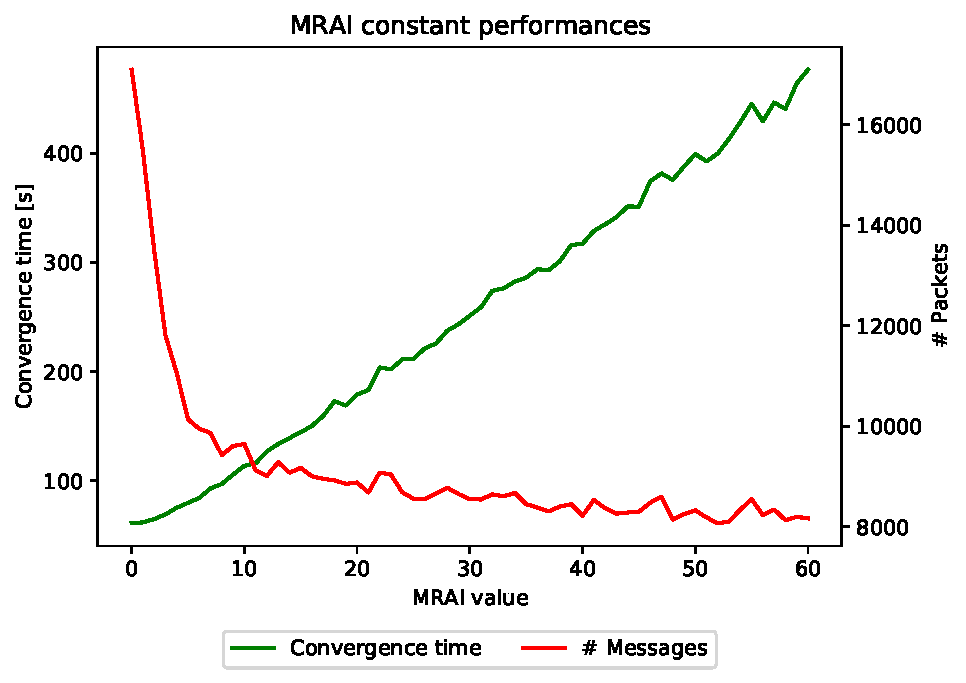
\includegraphics[width=\textwidth]{images/internet_like/1000/constantMRAI/internet_like-constant_mrai_evolution.pdf}
		 \caption{Network performances, messages VS convergence time with different
			\ac{MRAI} values}
         \label{fig:internet_like_1000_constant_evolution_evolution}
     \end{subfigure}
     \hfill
     \begin{subfigure}[b]{0.49\textwidth}
         \centering
         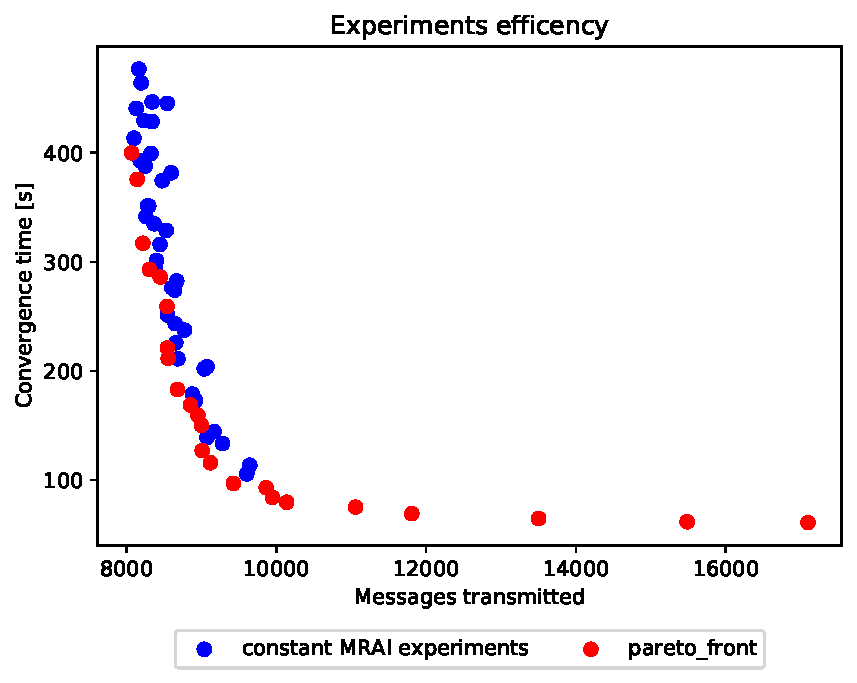
\includegraphics[width=\textwidth]{images/internet_like/1000/constantMRAI/internet_like-constant.pdf}
		 \caption{Pareto front of Messages VS Convergence time}
         \label{fig:internet_like_1000_constant_evolution_paretoFront}
     \end{subfigure}
		\caption{Evolution of the network performances on the \textbf{Internet Like} graph
			of \num{1000} nodes using a fixed \ac{MRAI} from \num{0} to \num{60} seconds.
			Each point is the average of \num{10} runs, in total has been executed
			\num{610} runs.\fxfatal{Adjust figure dimensions}}
        \label{fig:internet_like_1000_constant_evolution}
\end{figure}

As is possible to see in \Cref{fig:internet_like_1000_constant_evolution_evolution},
without \ac{MRAI} the convergence time would be low, dictated mostly by
network delays and processing time. With, on the other hand, an enormous amount
of messages.
Slightly increasing the \ac{MRAI} value, the number of messages fell down
reaching a constant value around \num{8000}, while the convergence time
continuously grows linearly, as it happened for the clique graph in \Cref{fig:clique_evolution}.
This continuous linear grow is dictated by the fact that nodes keep meaningful
information for more time before sharing them with their neighbourhood.

\Cref{fig:internet_like_1000_constant_evolution_paretoFront} represent the Pareto
front of those experiments.
The Pareto frontier is the set of values that are Pareto efficient, this concept
has been already used in engineering to define the set of best outcomes from
the trade-off of two different parameters \cite{goodarzi2014introduction}.
The majority of the points is concentrated on the left
of the chart, this means that few \ac{MRAI} values would give as a result
a high number of messages and a small convergence time.
While, multiple \ac{MRAI} values permits to have a concentration of results around the
same amount of messages transmitted.
This confirm the fact that \ac{MRAI} would not influence messages
after a certain threshold but only the convergence time.

The results of the same environment without \ac{IW} are showed in
\Cref{fig:internet_like_1000_constant_evolution_noIW}.

\begin{figure}[h]
     \centering
     \begin{subfigure}[b]{0.49\textwidth}
         \centering
         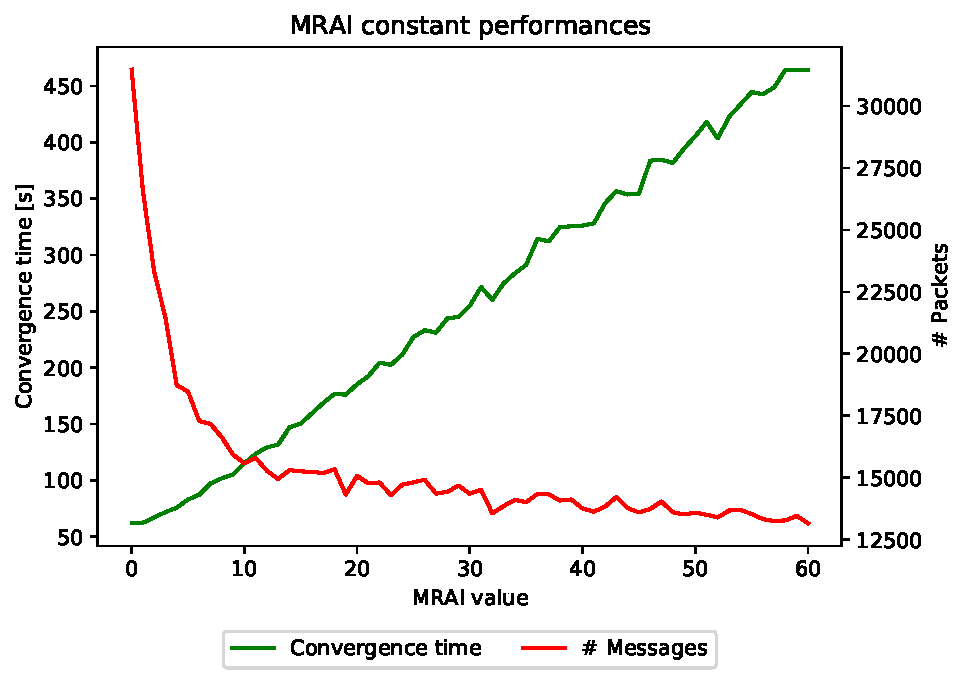
\includegraphics[width=\textwidth]{images/internet_like/1000/constantMRAI/internet_like-constant-noIW_mrai_evolution.pdf}
		 \caption{Network performances, messages VS convergence time with different
			\ac{MRAI} values}
         \label{fig:internt_like_1000_constant_noIW_evolution_evolution}
     \end{subfigure}
     \hfill
     \begin{subfigure}[b]{0.49\textwidth}
         \centering
         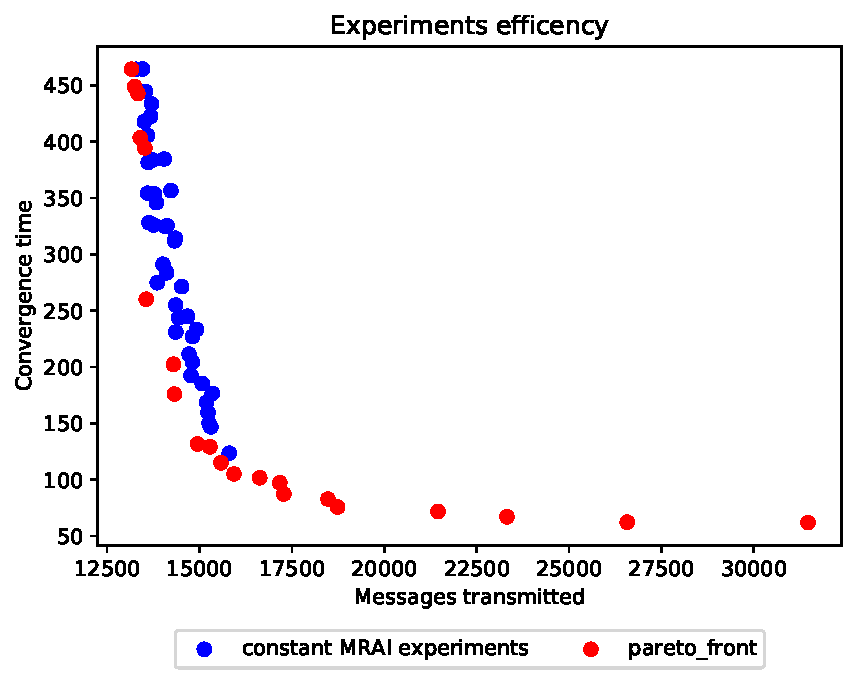
\includegraphics[width=\textwidth]{images/internet_like/1000/constantMRAI/internet_like-constant-noIW.pdf}
		 \caption{Pareto front of Messages VS Convergence time}
         \label{fig:internt_like_1000_constant_noIW_evolution_paretoFront}
     \end{subfigure}
		\caption{Evolution of the network performances on the \textbf{Internet Like} graph
			of \num{1000} nodes \textbf{without \ac{IW}}, \ac{MRAI} strategy
			\textit{Fixed}from \num{0} to \num{60} seconds. Total number of
			runs \num{610}, \num{10} for each \ac{MRAI} value used.\fxfatal{Adjust
			figure dimensions}}
        \label{fig:internet_like_1000_constant_evolution_noIW}
\end{figure}

Also in this case, comparing \Cref{fig:internet_like_1000_constant_evolution_noIW,fig:internet_like_1000_constant_evolution},
is possible to notice that \ac{IW}
helps to reduce the number of messages and the convergence time without impacting
the network performances trend.

The second strategy, the one dependant on the \ac{DPC}, produce the results
in \Cref{fig:internet_like_1000_dpc_evolution}
As mentioned before, all the timers are adjusted to respect the same mean as in
the \textit{fixed} \ac{MRAI} experiments.
For this reason points with the same \ac{MRAI} value are comparable one another.

\begin{figure}[h]
     \centering
     \begin{subfigure}[b]{0.49\textwidth}
         \centering
         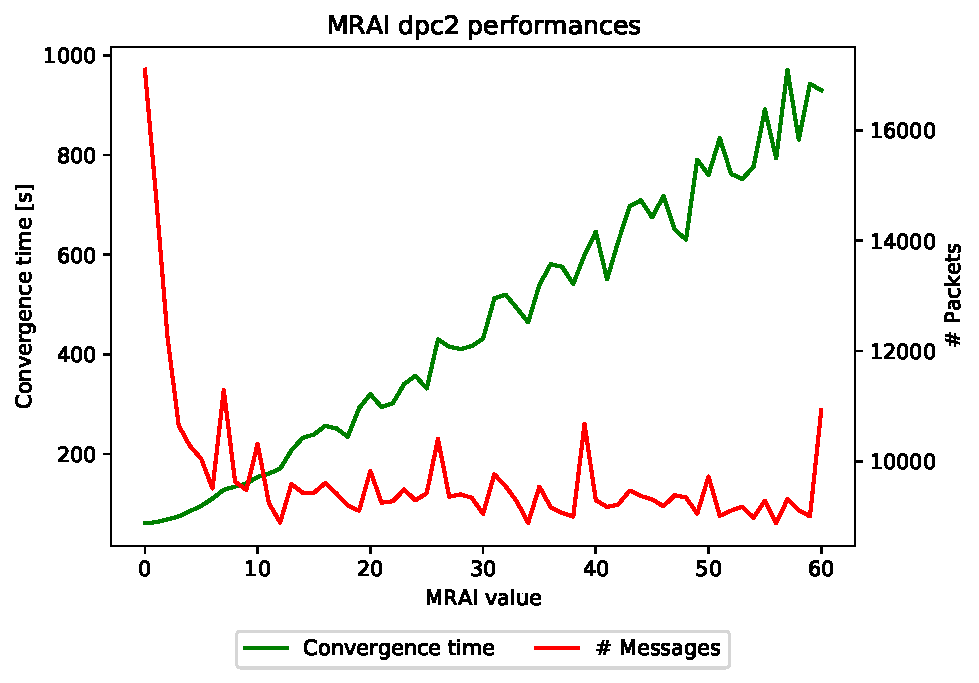
\includegraphics[width=\textwidth]{images/internet_like/1000/dpc/internet_like-DPC_mrai_evolution.pdf}
		 \caption{Network performances, messages VS convergence time with different
			\ac{MRAI} values}
         \label{fig:internt_like_1000_DPC_evolution_evolution}
     \end{subfigure}
     \hfill
     \begin{subfigure}[b]{0.49\textwidth}
         \centering
         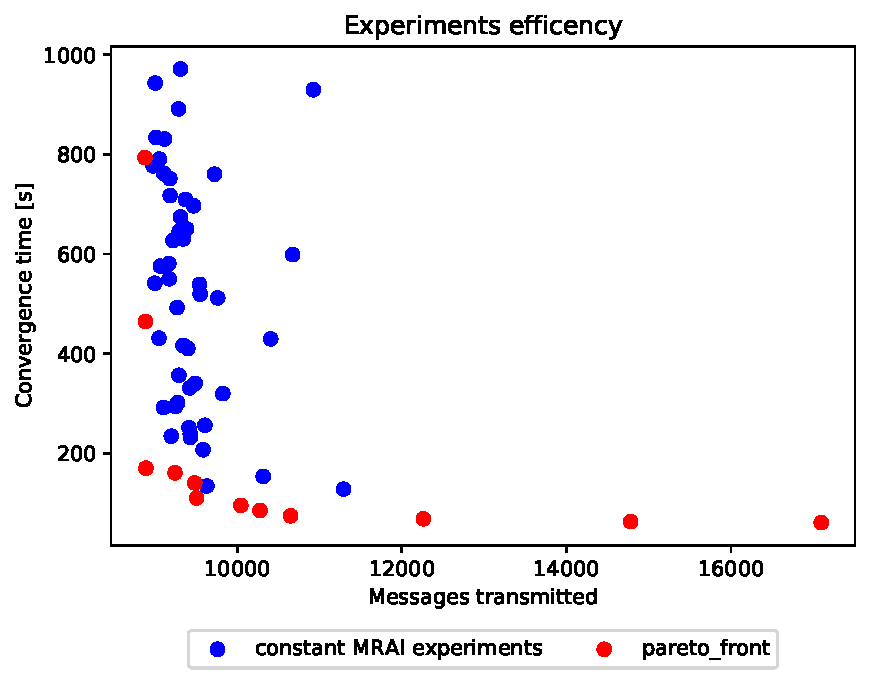
\includegraphics[width=\textwidth]{images/internet_like/1000/dpc/internet_like-DPC.pdf}
		 \caption{Pareto front of Messages VS Convergence time}
         \label{fig:internt_like_1000_DPC_evolution_paretoFront}
     \end{subfigure}
		\caption{Evolution of the network performances on the \textbf{Internet Like} graph
			of \num{1000} nodes using a \textit{DPC} \ac{MRAI} strategy
			with an $MRAI_{mean}$ from \num{0} to \num{60} seconds.}
        \label{fig:internet_like_1000_dpc_evolution}
\end{figure}

This second strategy leads to the performances showed in \Cref{fig:internet_like_1000_dpc_evolution},
where is possible to notice that the number of messages transmitted fell down
very quickly and it reaches the convergence value with an \ac{MRAI} value of
\num{10}.
But, it is also noticeable that there are a lot more spikes in this trend, that
deviate more from the constant value around \num{9000} messages.
And by consequence, the convergence time is affected by this behaviour.

Comparing \Cref{fig:internet_like_1000_dpc_evolution,fig:internet_like_1000_constant_evolution}
is possible to notice that the two strategies lead to a different trend.
Both are equal at the beginning with \ac{MRAI} equal \num{0}, but, after a while,
both the number of transmitted messages and the convergence time diverge.
The number of messages with the \ac{DPC} strategy variate more and it converges
around \num{9000} messages, while the \textit{fixed} strategy reaches \num{8000}
messages as stable point.
And, the convergence time with the second strategy grows more quickly.
This is caused by the central clique of tier-one nodes that have a high \ac{MRAI}
value.
The high \ac{MRAI} value is caused by the fact that all the leaves have \num{0.0}
as centrality producing an \ac{MRAI} value of \SI{0}{\second} and to respect
the $MRAI_{mean}$ value the central nodes need a massive value.
For example, with an $MRAI_{mean}$ of \SI{30}{\second} the node \num{1} (that is
one of the central clique nodes) has an \ac{MRAI} value of \SI{79.35}{\second} for all its
neighbours.


I compared those strategies performances using a box-plot, \Cref{fig:boxplot_internet_like_1000},
in a special case, the standard value of \ac{MRAI} is \SI{30}{\second} as described
in~\cite{rfc4271}, so I used it as \(MRAI_{mean}\).
I decided to execute \num{100} different runs for each strategy with the $MRAI_{mean}$
fixed to \SI{30}{\second}.

\begin{figure}[h]
     \centering
     \begin{subfigure}[b]{0.49\textwidth}
         \centering
         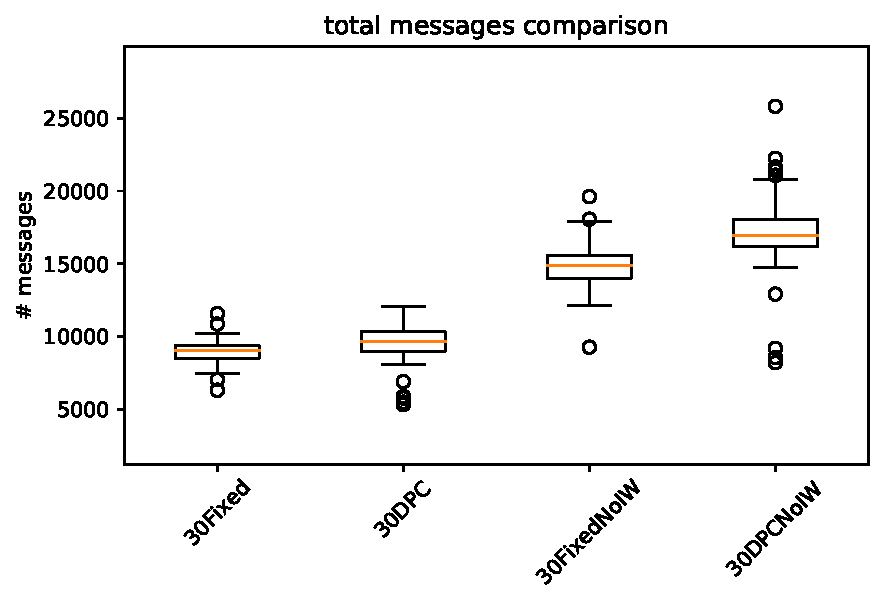
\includegraphics[width=\textwidth]{images/internet_like/1000/comparison/comparison_messages_boxplot.pdf}
		 \caption{Messages necessary to reach convergence
			with different \ac{MRAI} strategies}
         \label{fig:boxplot_internet_like_1000_messages}
     \end{subfigure}
     \hfill
     \begin{subfigure}[b]{0.475\textwidth}
         \centering
         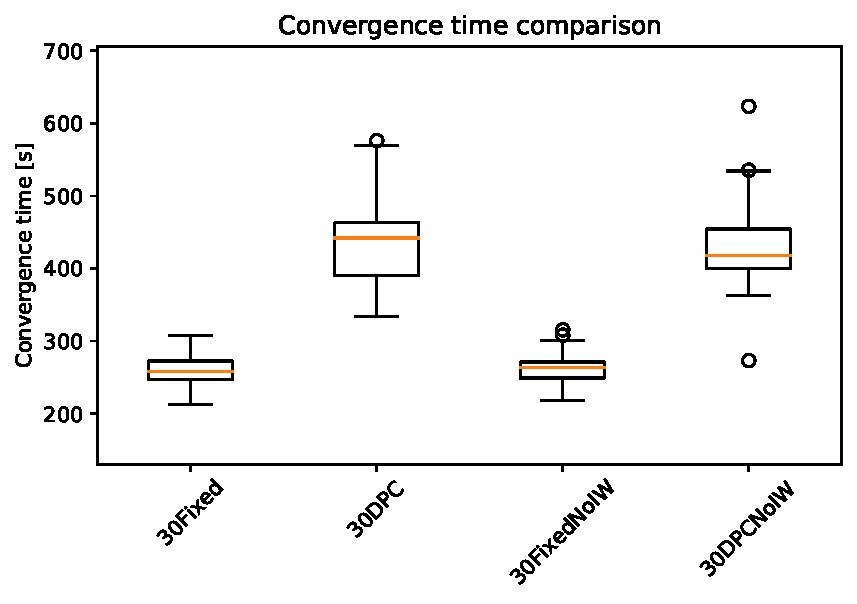
\includegraphics[width=\textwidth]{images/internet_like/1000/comparison/comparison_time_boxplot.pdf}
		 \caption{Time required to reach convergence
			with different \ac{MRAI} strategies}
         \label{fig:boxplot_internet_like_1000_time}
     \end{subfigure}
	 \caption{Network performances comparison with different \ac{MRAI} strategies,
		Graph internet like with \num{1000} nodes, \ac{MRAI} value
		\SI{30}{\second}, number of runs for each strategy \num{100}}
        \label{fig:boxplot_internet_like_1000}
\end{figure}

\Cref{fig:boxplot_internet_like_1000} permits to compare the two strategies already
mentioned.
The first plot, \Cref{fig:boxplot_internet_like_1000_messages}, represent
the number of messages transmitted by the \num{100} runs.
The two strategies, with the use of \ac{IW}, are really close one another on average,
with a difference of few thousands messages.
While, considering the time required to convergence, \Cref{fig:boxplot_internet_like_1000_time},
there are some huge difference between the two strategies.
The fact that the \ac{DPC} strategy requires almost the double of the
\textit{Fixed} one is not negligible.

In conclusion, I can confirm that the \ac{MRAI} strategy is one of the factors that
can influence the Network performances.

\section{Pareto Efficiency Front}
\label{sec:bgp_mrai_pareto_front}

The strategies exposed in \Cref{sec:bgp_mrai_strategy_dependance} are just few
of the available alternatives.
For this reason, I would like to explore the set of possibilities looking
for \ac{MRAI} configuration randomly generated.

I'm going to study the space of possibilities that are generated through the
Pareto efficiency plot and compare the results with the Pareto efficiency
graphs already presented in \Cref{sec:bgp_mrai_strategy_dependance}.
To permit this comparison I would set \ac{MRAI} randomly but, like for
the \ac{DPC} strategy, respecting the average required.

The environment used for those experiments is shown in \Cref{tbl:random_env}

\begin{table}[h]
	\begin{center}
	\begin{tabular}{ || m{4.9cm}| m{7.3cm} || } 
	\hline
	Property & Value \\ 
	\hline \hline
	Seeds & $[1, 10]$ \\ 
	\hline
	Signaling & \q{AW} \\
	\hline
		Withdraws delay & Uniform distribution between \SI{1}{\second} and \SI{60}{\second} \\ 
	\hline
		Implicit withdraw & Active \\ 
	\hline
		MRAI mean & $[0, 60]$ \\
	\hline
		MRAI values & Uniform distribution between \SI{1}{\second} and \SI{120}{\second} \\
	\hline
		Experiments per \ac{MRAI} mean & \num{10} \\
	\hline
	Link delay & Uniform distribution between \SI{0.012}{\second} and \SI{3}{\second} \\
	\hline

	\end{tabular}
\end{center}

	\caption{Random \ac{MRAI} environment properties}
	\label{tbl:random_env}
\end{table}

Thanks to this environment I'm going to run in total more than \num{600} complete
experiments.
For each \ac{MRAI} mean value, I will generate \num{10} different graphs with a random
\ac{MRAI} value assigned to each link.
I will then execute \num{10} different runs for each random graph that will produce
the average result of \num{1} experiment.
A single point is defined by the average convergence time and number of messages
of \num{10} runs.

In \Cref{fig:random_pareto_front} is possible to see all the \num{610} points
generated.

\begin{figure}[h]
    \centering
    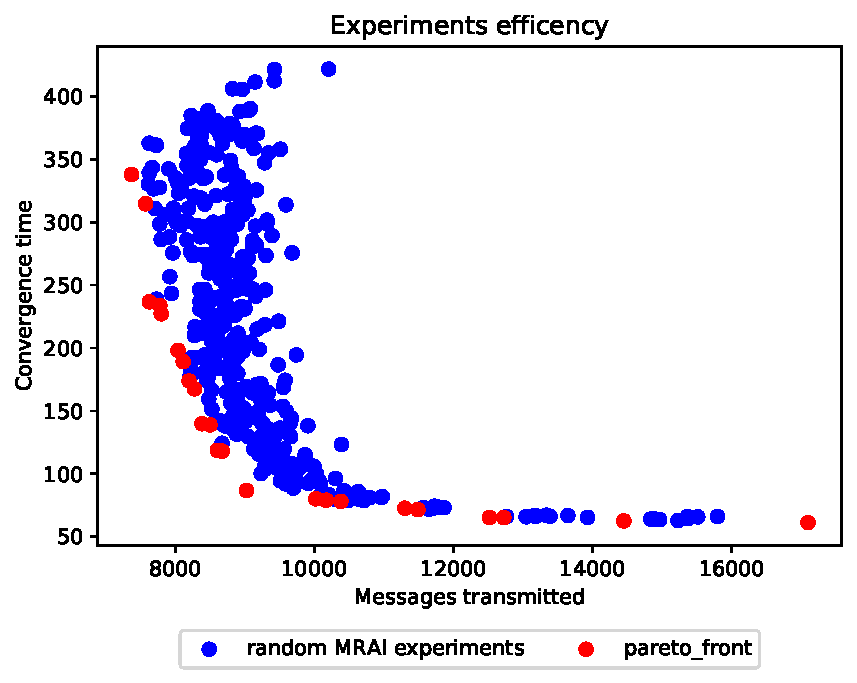
\includegraphics[width=.5\textwidth]{images/internet_like/1000/random.pdf}
	\caption{Pareto front generated by \num{610} experiments on an internet-like
	topology with \num{1000} nodes, \ac{MRAI} generated randomly and adapted to
		the mean, \num{610} total experiments, each point is the average of
		\num{10} points.}
    \label{fig:random_pareto_front}
\end{figure}

As we can see the trend in \Cref{fig:random_pareto_front} is similar to the one
that we saw for the same signal in \Cref{sec:bgp_mrai_strategy_dependance}.
For the majority of configurations, the number of messages transmitted is never
over \num{10000} but the time required to converge can grow over \SI{600}{\second}.

In \Cref{fig:pareto_comparison} is present a comparison between the random
experiments, the fixed \ac{MRAI} strategy and the \ac{DPC} strategy from
\Cref{fig:internet_like_1000_constant_evolution_paretoFront,fig:internt_like_1000_DPC_evolution_paretoFront}

\begin{figure}[h]
    \centering
    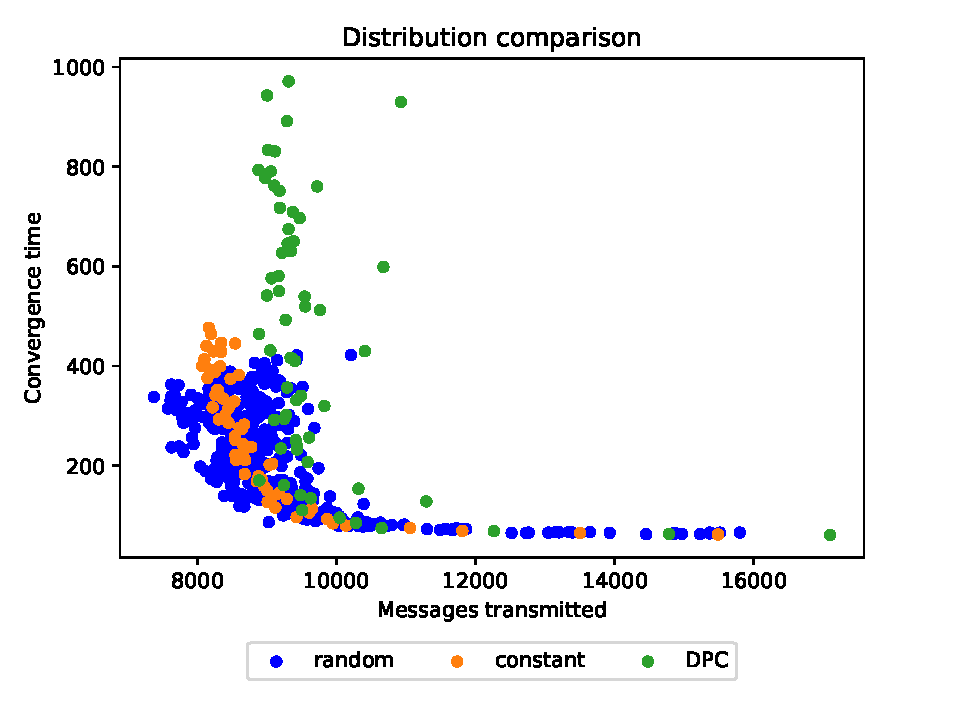
\includegraphics[width=.57\textwidth]{images/internet_like/1000/random_vs_all.pdf}
	\caption{Pareto front generated by \num{601} experiments on an internet-like
	topology with \num{1000} nodes, \ac{MRAI} generated randomly and adapted to
		the mean, vs fixed \ac{MRAI} strategy and \ac{DPC} \ac{MRAI} strategy.}
    \label{fig:pareto_comparison}
\end{figure}

As we can see in \Cref{fig:pareto_comparison} all the strategies have the same
behaviour, but is also possible to see that the random strategy is the only
one with experiments that produce less than \num{8000} messages.
This is important because it is the proof that better possibilities exists rather
that the classical one.

For this reason, \ac{MRAI} can be tuned to have a better trade-off between
the number of messages transmitted and convergence time.

\section{Signal dependence}
\label{sec:bgp_mrai_signal_dependance}

I would like to analyze how much the signal can impact the convergence performances
with the two different strategies of \Cref{sec:bgp_mrai_strategy_dependance}.

For this reason, I use the same environment described before and execute the
experiments with different input signals from the same node, \q{AWA}, \q{AWAW}
and \q{AWAWA}.

In those experiments plays a role also the \q{\textit{re-advertisement distribution}}
for the second and third \q{A}, it has been set to a uniform distribution
between \SI{1}{\second} and \SI{60}{\second}, like the \q{\textit{withdraw distribution}}.

For those experiments, I didn't evaluate the case with \ac{IW} deactivated.
Because, like we saw in
\Cref{fig:internet_like_1000_constant_evolution,fig:internet_like_1000_constant_evolution_noIW}
there is not a difference in terms of the trend.
Is straightforward to imagine that the performance of the following experiments
wouldn't have big differences in terms of tendency.

In \Cref{fig:internt_like_1000_evolution_AWA} is possible to see the evolution
for the signal \q{AWA}.

\begin{figure}[h]
     \centering
     \begin{subfigure}[b]{0.49\textwidth}
         \centering
         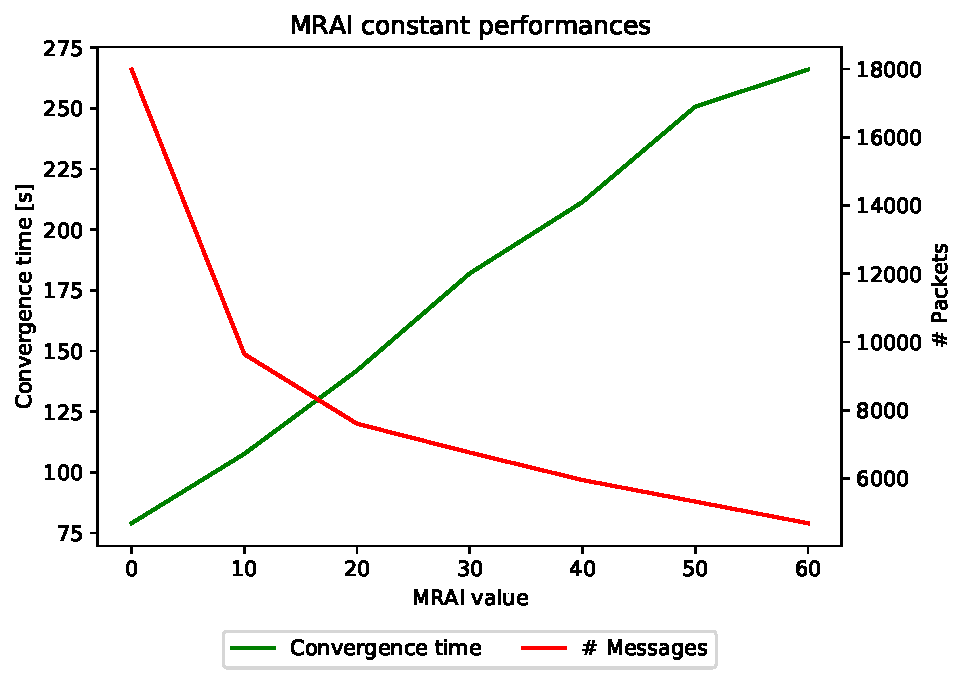
\includegraphics[width=\textwidth]{images/internet_like/1000/signals/AWA/constant/internet_like-constant_AWA_mrai_evolution.pdf}
		 \caption{Network performances, \textit{fixed} \ac{MRAI} strategy}
         \label{fig:internet_like_1000_fixed_AWA}
     \end{subfigure}
     \hfill
     \begin{subfigure}[b]{0.49\textwidth}
         \centering
         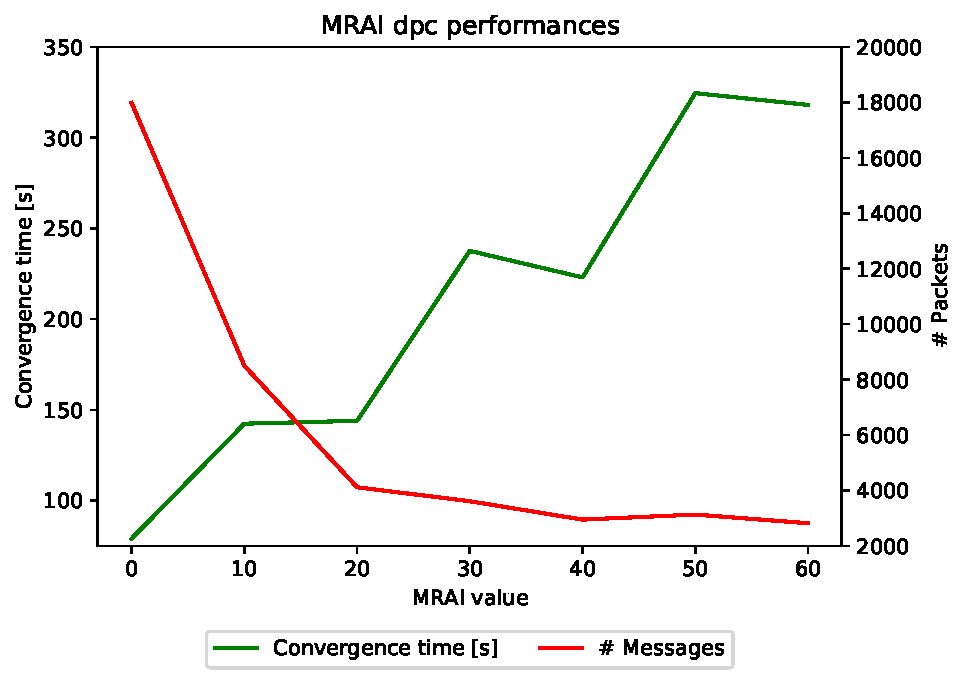
\includegraphics[width=\textwidth]{images/internet_like/1000/signals/AWA/dpc/internet_like-DPC_AWA_mrai_evolution.pdf}
		 \caption{Network performances, \ac{DPC} \ac{MRAI} strategy}
         \label{fig:internet_like_1000_dpc_AWA}
     \end{subfigure}
	 \caption{Network performances comparison with different \ac{MRAI} strategies,
		Graph internet like with \num{1000} nodes, signal \q{AWA}. Each point
		represent the average between \num{10} runs.}
        \label{fig:internt_like_1000_evolution_AWA}
\end{figure}

Is possible to notice in \Cref{fig:internt_like_1000_evolution_AWA} a big difference
compared to the plots in \Cref{fig:internet_like_1000_constant_evolution,fig:internet_like_1000_dpc_evolution}.
The \ac{DPC} strategy was able to outcome the standard \textit{fixed} strategy
over multiple prospective.
Analyzing \Cref{fig:internet_like_1000_dpc_AWA} is possible to see that
the red curve, the one that refers to the number of messages transmitted, has
a very fast fell.
With an average \ac{MRAI} timer \textit{of \SI{30}{\second}}
the number of messages is less than $1/4$ in respect of an \ac{MRAI} \textit{mean}
of \SI{0}{\second}.

The convergence time curve has a completely different trend in respect of the
previous experiments.
There are three steps in the trend, caused by the fact that
now the timer is able to effectively compress the signal.
\ac{MRAI} doesn't affect the first message, in this case the first \q{A} , but
it can affect the next two messages.
In fact, some nodes are able to cache both the \q{WA} part of the signal and
completely avoid sending anything at all, because they have already transmitted
the first \q{A}.
The complete compression of the signal \q{AWA} is \q{A}.
The other evolution, for the \q{AWAW} and \q{AWAWA} signals, are showed in
\Cref{fig:internt_like_1000_evolution_AWAW,fig:internt_like_1000_evolution_AWAWA}
Those valley are provoked by the gain in performances that the compression give
that overcomes the downside of having to make nodes wait longer.

Like before, comparing the standard \SI{30}{\second} fixed \ac{MRAI}, I executed
\num{100} different runs for each strategy and each different signal, the results
are showed in \Cref{fig:boxplot_internet_like_1000_time_allSignals}.

\begin{figure}[h]
     \centering
     \begin{subfigure}[b]{0.49\textwidth}
         \centering
         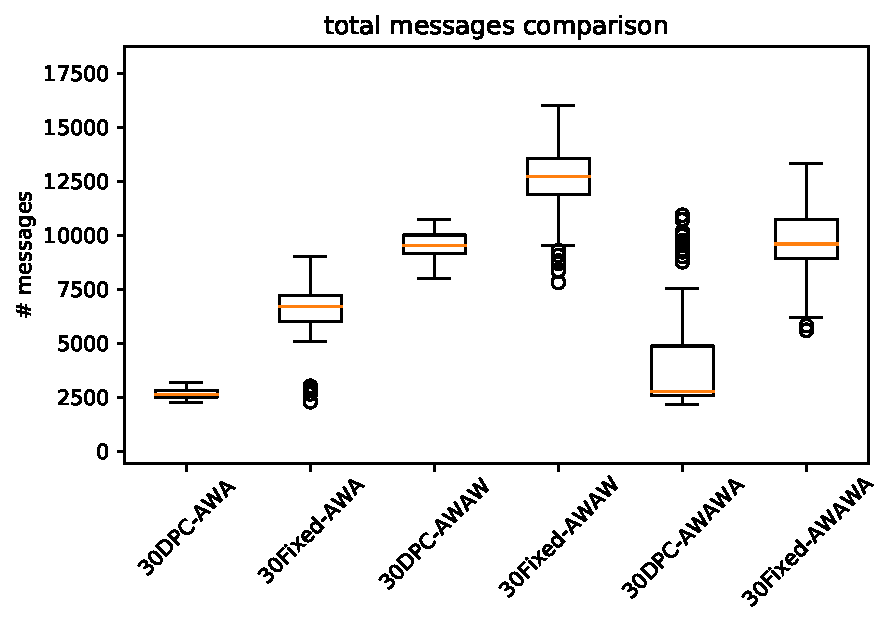
\includegraphics[width=\textwidth]{images/internet_like/1000/comparison/comparison_allSignals_messages_boxplot.pdf}
		 \caption{Network performances, messages necessary to reach convergence
			with different \ac{MRAI} strategies}
         \label{fig:boxplot_internet_like_1000_messages_allSignals}
     \end{subfigure}
     \hfill
     \begin{subfigure}[b]{0.49\textwidth}
         \centering
         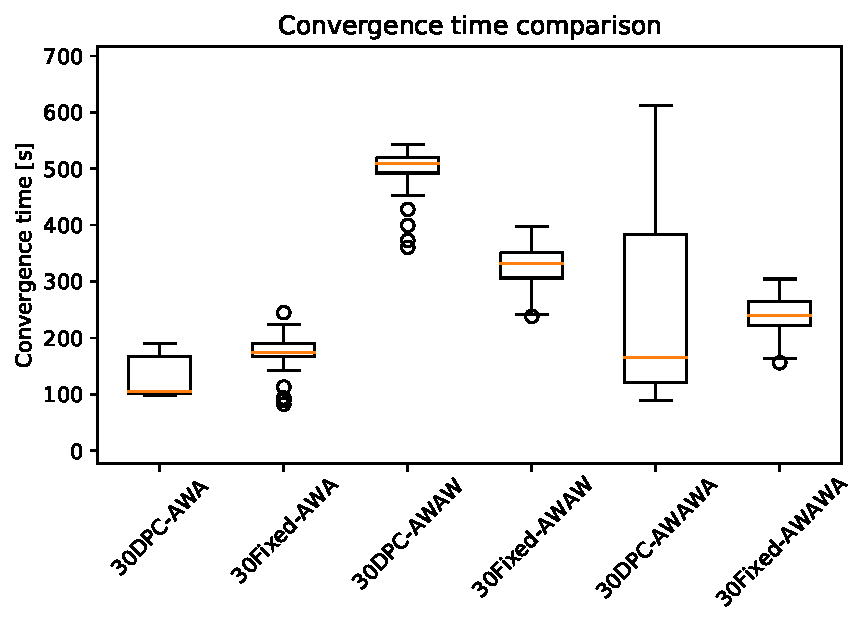
\includegraphics[width=\textwidth]{images/internet_like/1000/comparison/comparison_allSignals_time_boxplot.pdf}
		 \caption{Network performances, time required to reach convergence
			with different \ac{MRAI} strategies}
         \label{fig:boxplot_internet_like_1000_time_allSignals}
     \end{subfigure}
	 \caption{Network performances comparison with different \ac{MRAI} strategies,
		Graph internet like with \num{1000} nodes, \ac{MRAI} value
		\SI{30}{\second}, number of runs for each strategy \num{100}, signal \q{allSignals}}
        \label{fig:boxplot_internet_like_1000_allSignals}
\end{figure}

Is possible to notice in \Cref{fig:boxplot_internet_like_1000_allSignals} that
both the strategies have different performances in respect of the signal
produced by the single node source.
In particular, performances are better when the signal ends up with an \q{A}.
That's because, after the first \q{A}, giving a \ac{MRAI} timer long enough,
a node is able to compress a sequence that ends with another \q{A} to the
empty set and don't send anything more.
While if the sequence ends up with a \q{W} it has to, at least, send another
message to notify the withdraw.

Other than that is possible to notice that the \ac{DPC} techniques have better
results in terms of messages transmitted, while it could have a higher
convergence time.
This is caused, like before, by the high \ac{MRAI} values used by the most
central nodes.

In conclusion, there is an interaction between \ac{MRAI} and the sequence of messages
transmitted by the source node.
In particular more the timer is able to compress the sequence more the performances
can be improved.
Is not possible to increase the \ac{MRAI} timer indefinitely in order to catch
everything, because of the side effect on the convergence time.

\section{Position dependence}
\label{sec:position_dependance}

The last factor of influence for \ac{MRAI} that I would like to study is how much
the position of the signal source can influence the convergence.
The main hypothesis is that a node closer to the central clique, that generates
a signal would provoke a message storm bigger in respect of a node on the perimeter
of the network.
Because of the possibility from the nodes to catch the signal and compress it
before reaching the central clique.
A node near the central clique would provoke a case of \textit{Path exploration}
directly on the central clique.
This hypothesis could be true only if \ac{MRAI} is large enough to block the
storm near the source of the change, compressing the signal and exporting only
the correct information at the end of it.

\subsection{Different signal sources}
\label{subsec:different_destinations}

As first try, I have decided to analyse \num{10} different destinations chosen randomly
on the same graph, this graph is an Internet like topology with \num{1000} nodes.
I have then used the same environment with all the different destinations.
I also configured different \ac{MRAI} strategies, repeating the experiments for all of
them.
With this results is possible to analyze how different signal sources provoke
different network performances and also study how different \ac{MRAI} strategies
adapt to different nodes that provoke messages storms.

The environment used by those experiments is the one described in
\Cref{tbl:source_properties}.

\begin{table}[h]
	\begin{center}
	\begin{tabular}{ || m{4cm}| m{8cm} || }
	\hline
	Property & Value \\
	\hline \hline
	Seeds & $[1, 10]$ \\
	\hline
	Signaling & \q{AWAWA} \\
	\hline
		Withdraws delay & Uniform distribution between \SI{0.1}{\second} and \SI{60}{\second} \\
	\hline
	Announcement delay & Uniform distribution between \SI{0.1}{\second} and \SI{60}{\second} \\
	\hline
	Link delay & Uniform distribution between \SI{0.0001}{\second} and \SI{0.5}{\second} \\
	\hline
			\(MRAI_{mean}\) & $[0, 60]$ with steps of \num{10} \\
	\hline
		Random nodes & \num{10} \\
	\hline
		\ac{MRAI} strategies & Fixed \ac{MRAI}, \ac{DPC}, reverse \ac{DPC} \\
	\hline
	\end{tabular}
\end{center}

	\caption{Different signal sources environment properties}
	\label{tbl:source_properties}
\end{table}

Like mentioned in \Cref{tbl:source_properties} I decided to use another
\ac{MRAI} strategy and look forward to its performances.
That strategy is the reverse of the one base on the \ac{DPC} described in
\Cref{subsec:bgp_mrai_dpc}.
I will use a higher \ac{MRAI} for the first part of the graph and a smaller
one in the descending phase.

In total, I have executed \num{700} runs for each \ac{MRAI} strategy with the
\num{10} different signal sources.
The resulting network evolution with different \ac{MRAI} values is shown in
\Cref{fig:different_destinations}.
Each point of \Cref{fig:different_destinations_all} represents the average
of the \num{10} runs executed for the specific destination with that \ac{MRAI}
configuration.
\Cref{fig:different_destinations_mean} shows the average result
obtained from all the \num{10} different destinations for a specific \ac{MRAI}
strategy.

\begin{figure}[h]
     \centering
     \begin{subfigure}[b]{0.49\textwidth}
         \centering
         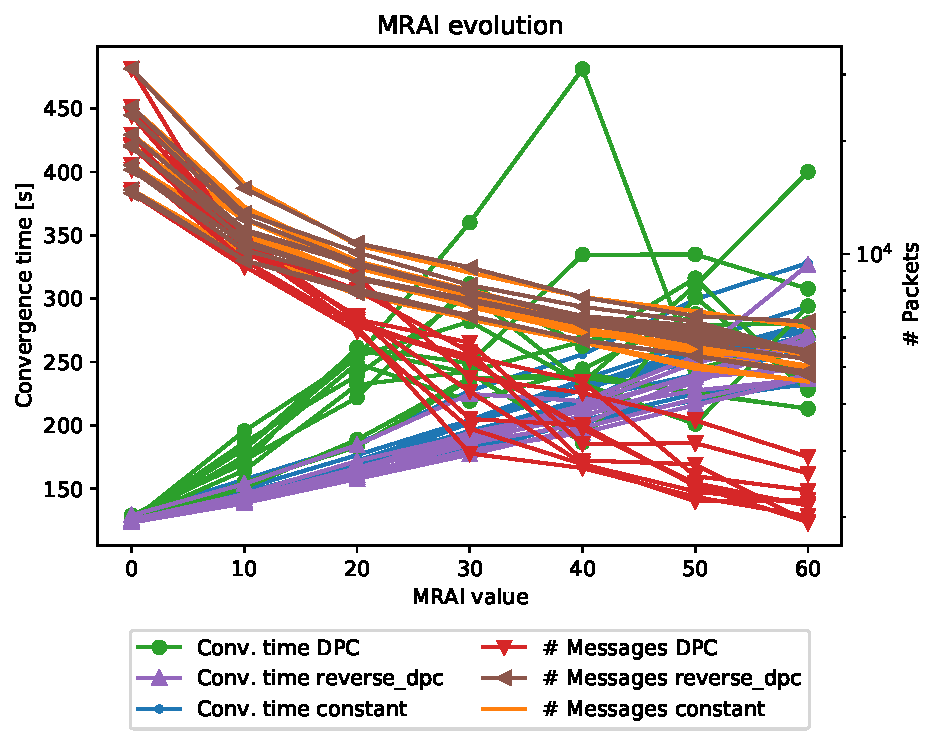
\includegraphics[width=\textwidth]{images/position/different_destinations-1000_all.pdf}
		 \caption{Network performance evolution of all the \num{10} different signal sources
			with the different \ac{MRAI} strategies}
         \label{fig:different_destinations_all}
     \end{subfigure}
     \hfill
     \begin{subfigure}[b]{0.49\textwidth}
         \centering
         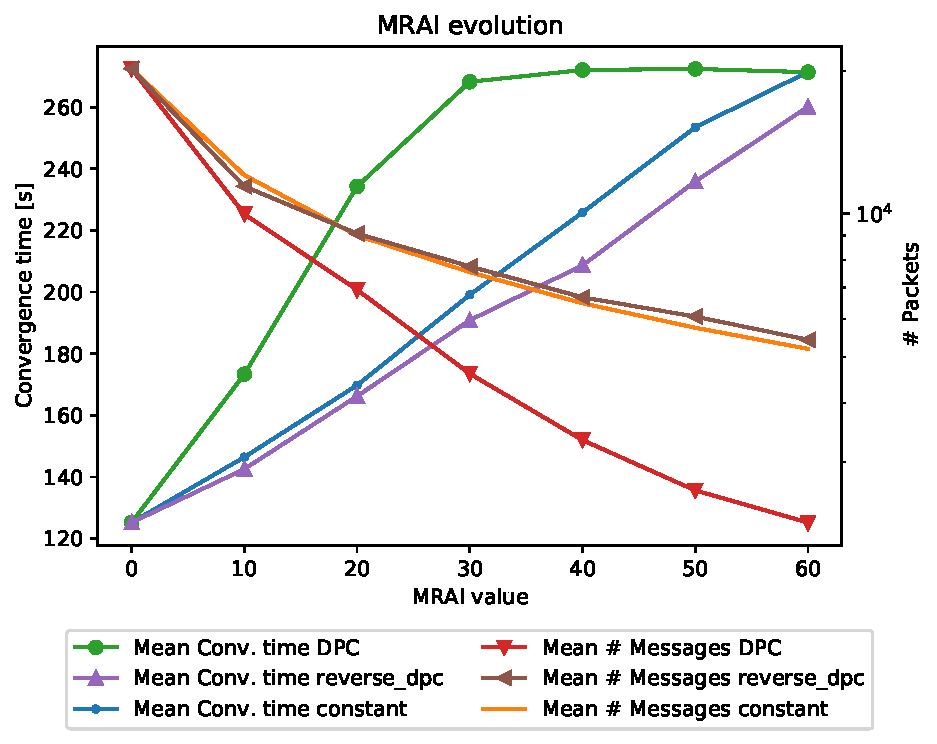
\includegraphics[width=\textwidth]{images/position/different_destinations-1000_mean.pdf}
		 \caption{Average of the network performances of \num{10} different
			signal sources are chosen with different \ac{MRAI} strategies}
         \label{fig:different_destinations_mean}
     \end{subfigure}
	 \caption{Network performances given \num{10} different signal sources chosen
		randomly on an Internet like graph of \num{1000} nodes, with different
		\ac{MRAI} strategies used, fixed, \ac{DPC}, Reverse \ac{DPC}, and
		different \ac{MRAI} mean values. Each point represent the average of
		\num{10} different runs.}
	 \label{fig:different_destinations}
\end{figure}

\Cref{fig:different_destinations} shows how, changing the source of the signal,
also changes the network performances with multiple \ac{MRAI} values.
Notice that the second y-axis, the one that represents the number of packets
transmitted, is in log scale.
We can use the plot in \Cref{fig:different_destinations_all} to see the
differences between one destination and the others, while \Cref{fig:different_destinations_mean}
expose the differences between the different strategies.
We can see in \Cref{fig:different_destinations_all} that all the \num{10} destinations
cause a similar behaviour with the fixed strategy and the reverse \ac{DPC}, both
in terms of messages transmitted and also convergence time.
In both techniques, the difference between the \num{10} destinations in terms of
convergence time is a few tens of seconds, with linear growth.
Thanks to \Cref{fig:different_destinations_mean} is possible to see that the
number of messages reaches a convergence value between \num{5000} and
\num{6000}.
The \ac{DPC} strategy seems to bee more volatile with the growth of \ac{MRAI},
both in terms of messages and also convergence time.
In \Cref{fig:different_destinations_all}, from the multiple green spikes is possible to see
that the position of the source is highly affective using this strategy.
In terms of messages transmitted the \ac{DPC} strategy always goes better than
the other two strategies, respecting the trend in \Cref{sec:bgp_mrai_signal_dependance}.

We can conclude that the position of the source can influence the behaviour
of \ac{MRAI}, it is more influent when the strategy used relies on topological
information, like the \ac{DPC} strategy.
But, the chose of the strategy is more influent, the number of messages transmitted
by the \ac{DPC} strategy are always less than the one transmitted by the other
two strategies, for every destination.

\subsection{Hierarchical influence}
\label{subsec:hierarchical_influence}

What about the position in the hierarchy?
Internet is very strong hierarchical graph, \Cref{fig:internet_topology_hierarchical}
is an example with a small set of nodes but is possible to distinguish different levels
in the graph.
If we take the central clique as the root of the graph then all the nodes will
be at a certain distance (in terms of hops) from it.

The question is: Nodes that are on the same hierarchical level reacts in the same way?

To analyze this possibility I decided to take randomly \num{3} nodes from each
hierarchical level of an Internet-like topology of \num{1000} nodes, the number
of levels in this graph is \num{4}.
The total number of destinations is \num{12} and for each one of them I executed
an experiment with multiple \ac{MRAI} strategies and different \(MRAI_{mean}\)
values.

The properties of this environment are summarized in \Cref{tbl:hierarchical_properties}.

\begin{table}[h]
	\begin{center}
	\begin{tabular}{ || m{4cm}| m{8cm} || } 
	\hline
	Property & Value \\ 
	\hline \hline
	Seeds & $[1, 10]$ \\ 
	\hline
	Signaling & \q{AWAWAWAW} \\
	\hline
		Withdraws delay & Uniform distribution between \SI{0.1}{\second} and \SI{5}{\second} \\ 
	\hline
	Announcement delay & Uniform distribution between \SI{0.1}{\second} and \SI{5}{\second} \\ 
	\hline
	Link delay & Uniform distribution between \SI{0.0001}{\second} and \SI{0.5}{\second} \\
	\hline
		MRAI & $[0, 60]$ with steps of \num{10} \\
	\hline
		Number of levels & \num{4} \\
	\hline
		Random dst per level & \num{3} \\
	\hline
		\ac{MRAI} strategies & \ac{DPC}, reverse \ac{DPC} \\
	\hline
	\end{tabular}
\end{center}

	\caption{Hierarchical experiments environment properties}
	\label{tbl:hierarchical_properties}
\end{table}

Given that, I am evaluating the impact of nodes by their distance from
the center of the network, it is a good way also to test strategies
which goal is to enforce those points.
For this reason, I chose those two strategies that relies on the centrality of the nodes.

The results in \Cref{fig:different_levels} shows the different evolution of
the random sources for each different level, from the first to the fourth.

\begin{figure}[h]
     \centering
     \begin{subfigure}[b]{0.49\textwidth}
         \centering
         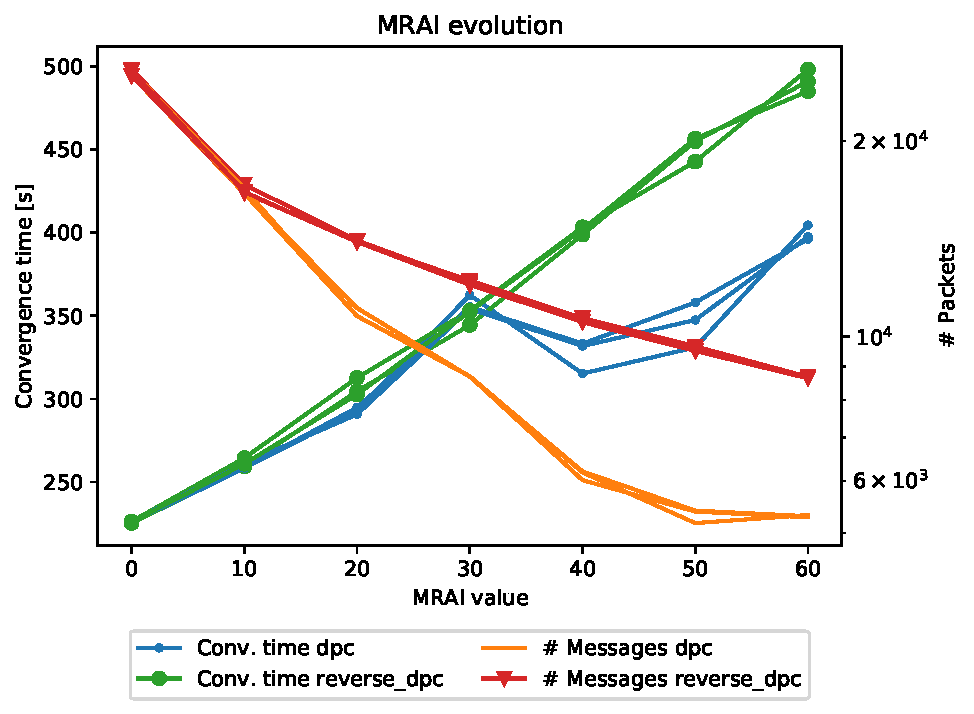
\includegraphics[width=\textwidth]{images/hierarchy/different_levels-1000_hier_1_all.pdf}
		 \caption{Network performances evolution of all the \num{3} different signal sources
			with the different \ac{MRAI} strategies at the hierarchical level \num{1}}
         \label{fig:different_levels_1}
     \end{subfigure}
	 \hfill
     \begin{subfigure}[b]{0.49\textwidth}
         \centering
         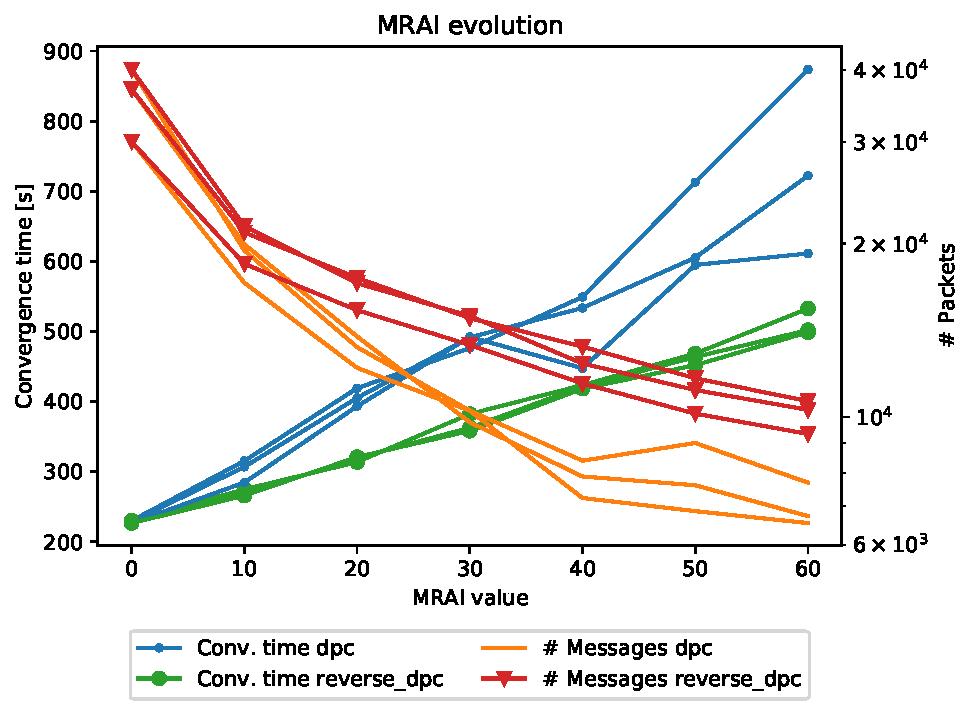
\includegraphics[width=\textwidth]{images/hierarchy/different_levels-1000_hier_2_all.pdf}
		 \caption{Network performances evolution of all the \num{3} different signal sources
			with the different \ac{MRAI} strategies at the hierarchical level \num{2}}
         \label{fig:different_levels_2}
     \end{subfigure}
     \begin{subfigure}[b]{0.49\textwidth}
         \centering
         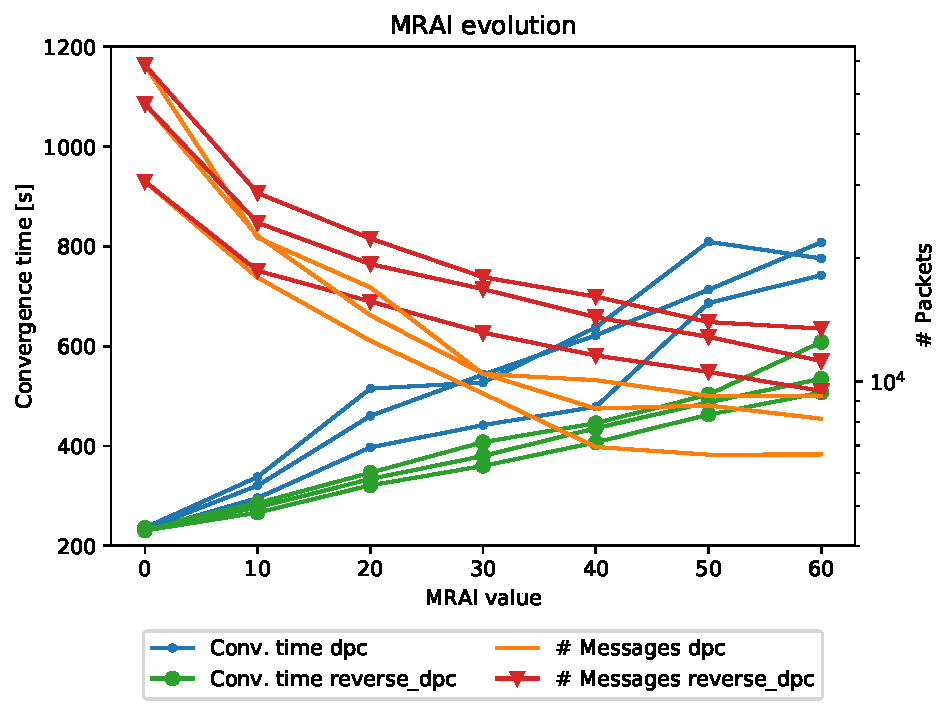
\includegraphics[width=\textwidth]{images/hierarchy/different_levels-1000_hier_3_all.pdf}
		 \caption{Network performances evolution of all the \num{3} different signal sources
			with the different \ac{MRAI} strategies at the hierarchical level \num{3}}
         \label{fig:different_levels_3}
     \end{subfigure}
	 \hfill
     \begin{subfigure}[b]{0.49\textwidth}
         \centering
         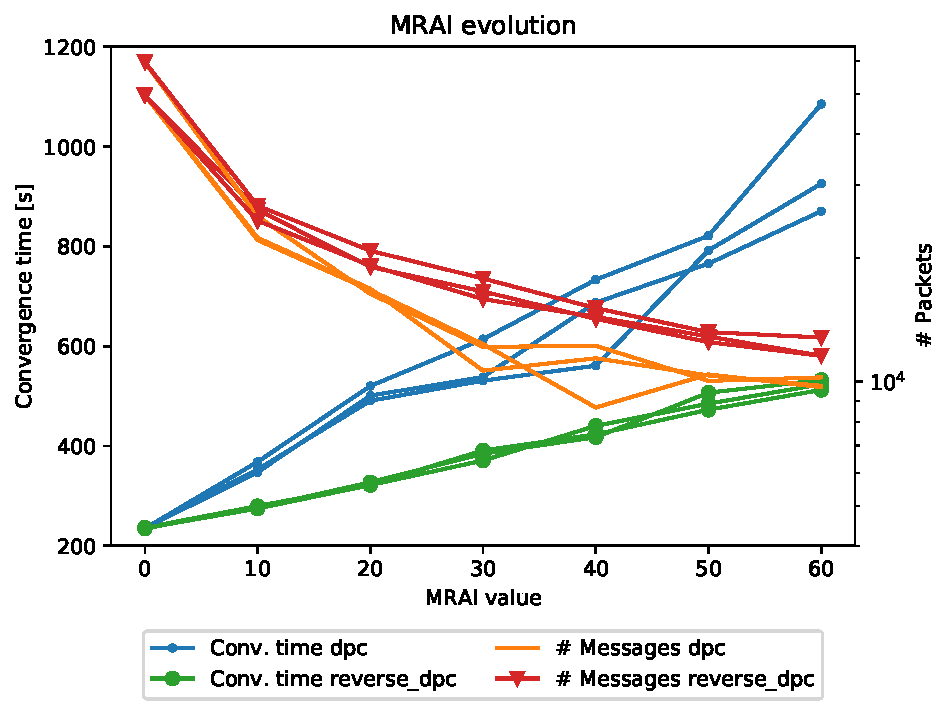
\includegraphics[width=\textwidth]{images/hierarchy/different_levels-1000_hier_4_all.pdf}
		 \caption{Network performances evolution of all the \num{3} different signal sources
			with the different \ac{MRAI} strategies at the hierarchical level \num{4}}
         \label{fig:different_levels_4}
     \end{subfigure}
     \hfill
	 \caption{Network performances given \num{3} different signal sources chosen
		randomly for each level of the Internet like graph, number of nodes
		\num{1000}, number of levels \num{4}, different \ac{MRAI} strategies
		\ac{DPC} and reverse \ac{DPC} \fxfatal{Adjust messages ticks}}
	 \label{fig:different_levels}
\end{figure}

In \Cref{fig:different_levels} is possible to see the evolution of the network
with different source nodes from different levels and how \ac{MRAI} influence
the network performances.
Starting from the first level in \Cref{fig:different_levels_1}, where the source
node is directly connected with a node of the central clique we can see different
important things.
First of all, the variance between the three different sources is very small,
both in terms of messages transmitted and also convergence time.
Both the techniques, \ac{DPC} and the reverse of it, in terms of messages
transmitted starts from a value around \num{25000} with \ac{MRAI} equal to
\SI{0}{\second} and both reaches a value under \num{10000} units.
In terms of convergence time, the reverse strategy grows linearly as expected
while the \ac{DPC} technique is able to gain a strong reduction thanks to
the efficient messages compression.

Going to the second and third level, respectively in
\Cref{fig:different_levels_2,fig:different_levels_3}, we can see that there
is an increase of the variance between the single source trends, both in terms
of messages and also convergence time.
Also, the number of messages transmitted slowly increases, at the beginning the
number of messages reaches \num{60000} units converging around \num{10000}.

In \Cref{fig:different_levels_4} we can see the worst-case scenario, not in
terms of variance between the sources, but in this case, we have the worst
performances.
The convergence time grows even over \SI{1000}{\second} for the \ac{DPC} strategy.
While the number of messages transmitted with \ac{MRAI} equal to \SI{0}{\second}
touches \num{60000} reaching a convergence value slightly over \num{10000}.

The influence that the position of the source nodes has to
a hierarchical graph like the Internet is clear.
The performances with \ac{MRAI} at \SI{0}{\second} are only attributable to the
strategic position of the source node.
But, while \ac{MRAI} grows, the position plays a central role on the performances.
Nodes closer to the central clique have less space to provoke fluctuations
in terms of possible paths, causing a less active effect of the \textit{Path exploration}
problem.
Our initial hypothesis is proven to be wrong, nodes that are farthest are more incline
to provoke a more intense path fluctuation and by consequence there are inferior
performances.

Another hypothesis is that there is a difference in the single nodes based
on the position in the topology.
Nodes that are more central, if the signal comes from closer nodes could
react with a more explosive \textit{Path exploration} behaviour.
If the signal comes from the periphery of the network, the other side of
it could require more time to converge in respect of a signal that starts
near the center.

To prove that hypothesis I decided to use the data from this set of experiments
with \ac{MRAI} value equal to \SI{30}{\second}.
I calculated for each node the average performances, based on the level, convergence
time, number of messages necessary to reach the convergence state and the \ac{DPC}
centrality value.
I have then grouped nodes that are at the same distance from the source, to
calculate the distance I used the distance in terms of hops in the \textit{Best
Path}.
I then calculated the average performances of each group.
The results are showed in \Cref{fig:different_levels_comparison}.

\begin{figure}[h]
     \centering
     \begin{subfigure}[b]{0.49\textwidth}
         \centering
         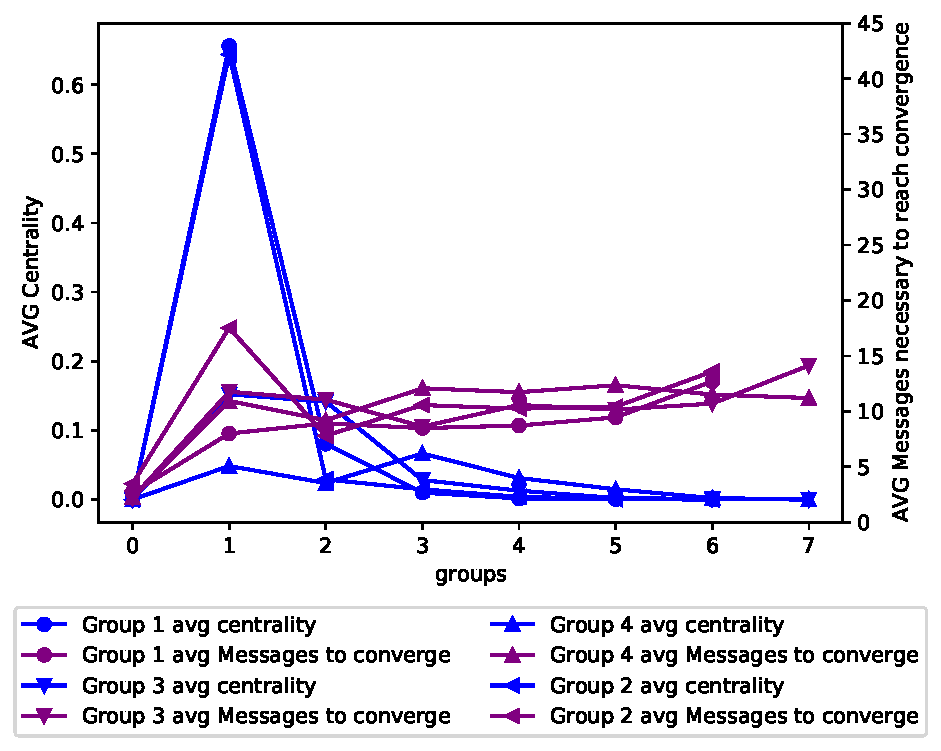
\includegraphics[width=\textwidth]{images/hierarchy/dpc_all_levels_comparison_centVSmsg.pdf}
		 \caption{\ac{DPC} strategy, number of messages necessary on
			average to reach convergence, levels comparison}
         \label{fig:different_levels_comparison_dpc_msg}
     \end{subfigure}
	 \hfill
     \begin{subfigure}[b]{0.49\textwidth}
         \centering
         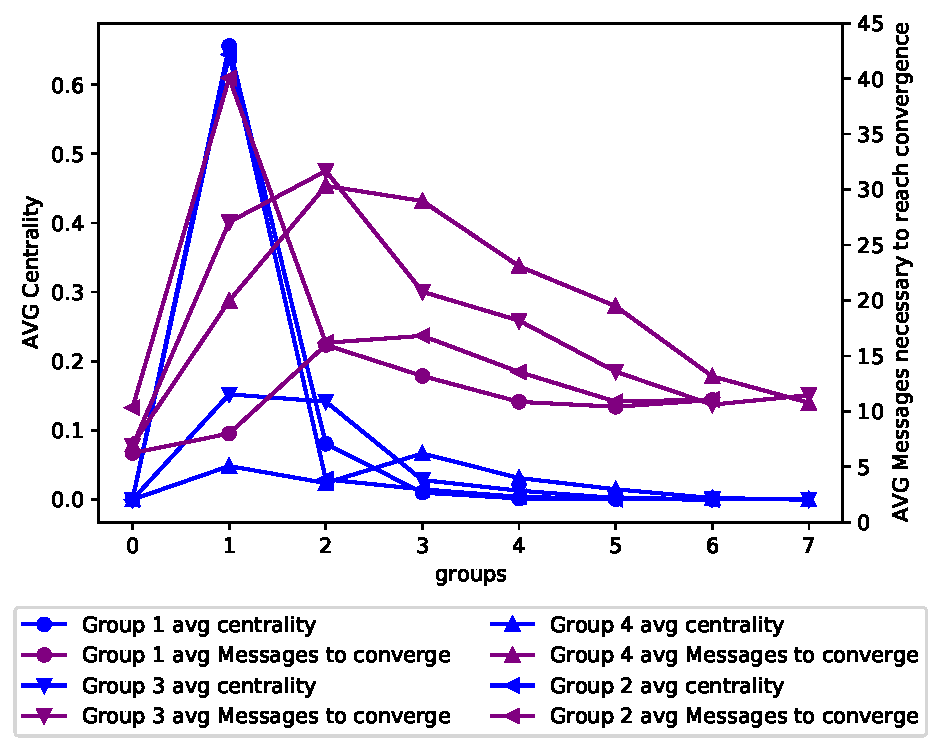
\includegraphics[width=\textwidth]{images/hierarchy/reverse_dpc_all_levels_comparison_centVSmsg.pdf}
		 \caption{reverse \ac{DPC} strategy, number of messages necessary on
			average to reach convergence, levels comparison}
         \label{fig:different_levels_comparison_reverse_dpc_msg}
     \end{subfigure}
     \begin{subfigure}[b]{0.49\textwidth}
         \centering
         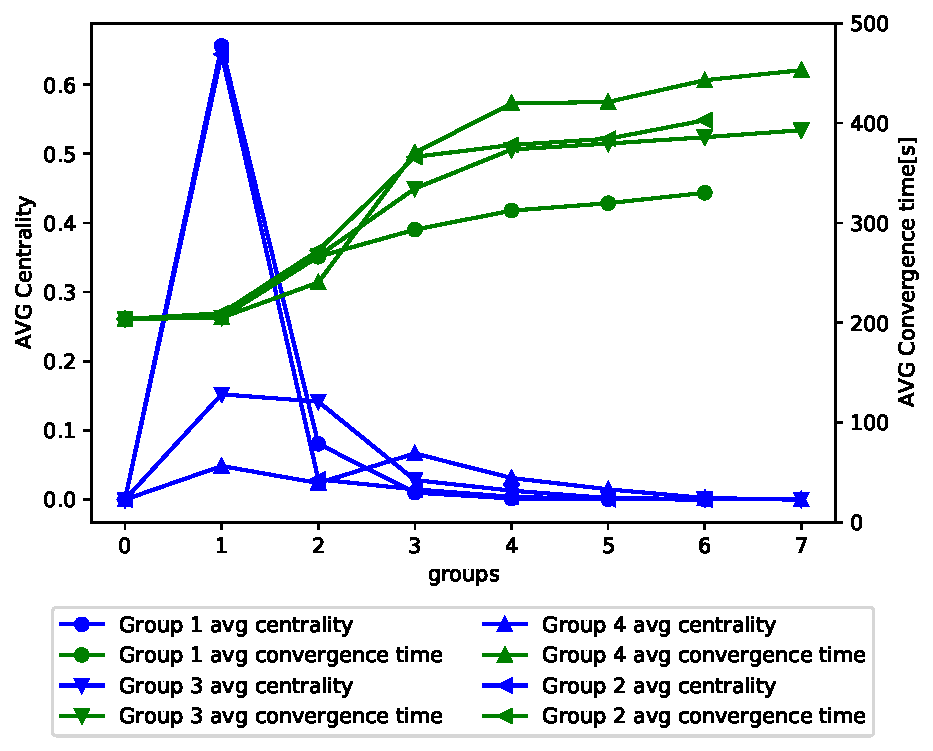
\includegraphics[width=\textwidth]{images/hierarchy/dpc_all_levels_comparison_centVStime.pdf}
		 \caption{\ac{MRAI} strategy \ac{DPC}, convergence time levels comparison}
         \label{fig:different_levels_comparison_dpc_time}
     \end{subfigure}
	 \hfill
     \begin{subfigure}[b]{0.49\textwidth}
         \centering
         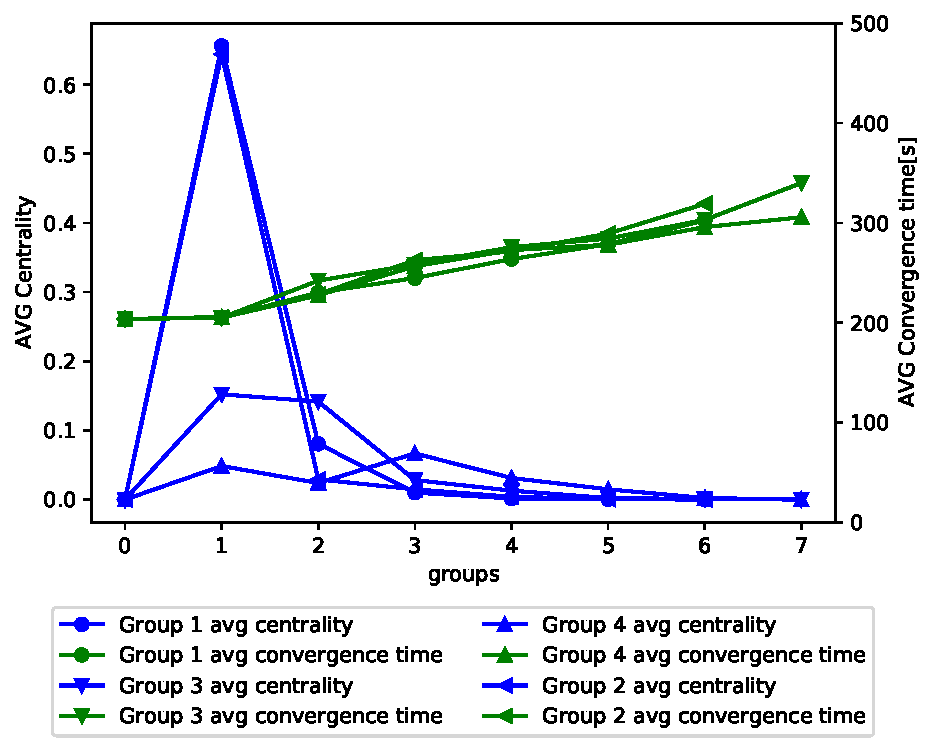
\includegraphics[width=\textwidth]{images/hierarchy/reverse_dpc_all_levels_comparison_centVStime.pdf}
		 \caption{\ac{MRAI} strategy reverse \ac{DPC}, convergence time levels comparison}
         \label{fig:different_levels_comparison_reverse_dpc_time}
     \end{subfigure}
     \hfill
	 \caption{Internet like topology of \num{1000} nodes grouped by the distance
	 from the signal source, different level comparison with \ac{MRAI} strategy
		\ac{DPC} and reverse \ac{DPC}, \ac{MRAI} value equal to \SI{30}{\second}}
	 \label{fig:different_levels_comparison}
\end{figure}

In \Cref{fig:different_levels_comparison} is possible to see an analysis of the
average nodes performances grouped by the distance from the source of the signal.
Those performances are taken from the case where \(MRAI_{mean}\) is equal to
\SI{30}{\second}.
On the left side, in
\Cref{fig:different_levels_comparison_dpc_msg,fig:different_levels_comparison_dpc_time}
are showed the performances of the nodes that uses the \ac{DPC} strategy.
While, on the other side, \Cref{fig:different_levels_comparison_reverse_dpc_msg,fig:different_levels_comparison_reverse_dpc_time},
expose the performances in case of the reverse \ac{DPC} strategy.

In all the plots in \Cref{fig:different_levels_comparison} the blue line
represents the average normalized centrality of the different nodes groups at different
levels.
Is possible to see that in the case that the nodes are in the first or the
second level the nodes with the highest average centrality are the nearest ones.
While if the node is far away from the central clique the nodes with the
higher average centrality are in the second or third group.
The values for those groups are low because of the high number of nodes
in those groups, most of them having a small centrality value.
The centrality refers to the first y-axis on the left.

The two plots in \Cref{fig:different_levels_comparison_dpc_msg,fig:different_levels_comparison_reverse_dpc_msg},
respectively the \ac{DPC} case and the reverse \ac{DPC},
show the average number of messages required by each group of nodes to reach
the convergence state.
The main difference between them is in the number of messages experienced by
the nodes near the source.
In the \ac{DPC} case, the value remains stable around \num{10} messages, while,
with the reverse strategy, this number explodes up to \num{40} messages because
of the \textit{Path exploration} problem provoked by the ascending part of the graph.

Is possible to notice that some of the lines end up at the $6^{th}$ hop instead
of the $7^{th}$, that's because for the level \num{1} and \num{2} there are
no best paths to the destination that goes over the \num{6} hops.

The convergence time is presented in
\Cref{fig:different_levels_comparison_dpc_time,fig:different_levels_comparison_reverse_dpc_time}.
Is easily noticeable that with the \ac{DPC} strategy after the
more central groups there is a separation between the lines, but the trends
are the same.
The convergence time slowly increases in farthest nodes, thanks to the particular
\ac{MRAI} strategy that permits to wait for enough time to receive all the information
necessary.
This is also the reason for the small variance in terms of messages transmitted.
With the reverse \ac{DPC} strategy, on the other hand, is possible to have a
more stable trend in the convergence time that linearly grows.
This linear trend is caused by the fact that nodes could end up to send more
\ac{ADV} in order to correct a non best route.
This is one of the consequences of the \textit{Path Exploration} problem in
the central nodes.

Is then possible to conclude that the position of the node can highly impact
the \ac{MRAI} behaviour, signals from the periphery of the network can more
easily cause \ac{ADV} storms if \ac{MRAI} is not large enough to catch them.
Other than that, the position can influence the performances by itself, but
\ac{MRAI} can help to reduce the number of messages paying a higher convergence
time.
The single nodes load can be affected by both the position and the strategy
used, a strategy that better reacts to the \textit{Path Exploration} problem
can prevent huge loads on the central nodes.

%\begin{itemize}
%    \item And how much is influencing the position?
%    \item Hierarchically?
%\end{itemize}
